\documentclass[11pt,reqno]{amsart}

\usepackage{amsthm,amsmath,amssymb}
\usepackage{mathtools}
\usepackage{proof}
\usepackage{xcolor}
\usepackage{graphicx}
\usepackage[T1]{fontenc}
\usepackage{courier}
\usepackage{hyperref}
\hypersetup{
    hidelinks=true
}
\usepackage{array}
\usepackage{multirow}
\usepackage{listings}
\lstset{basicstyle=\ttfamily\tiny, columns=fullflexible, language=Python, morekeywords={logical_and, log, exp, dot, sqrt, ones, identity}}
\newcommand{\code}[1]{\texttt{#1}}
\newcommand\MyBox[2]{
  \fbox{\lower0.75cm
    \vbox to 1.7cm{\vfil
      \hbox to 1.7cm{\hfil\parbox{1.4cm}{#1\\#2}\hfil}
      \vfil}%
  }%
}
\graphicspath{ {./} }

\begin{document}

\begin{center}
\large\textbf{Assignment 5 \\ DASC521 Fall 2019} \\
\normalsize\textbf{Introduction to Machine Learning \\  Erhan Tezcan 0070881 \\ 29.11.2019} \\
\end{center}

\section{Task}
We are given a univariate regression data set, which contains 272 data points about the duration of the eruption and waiting time between eruptions for the Old Faithful geyser in Yellowstone National Park, Wyoming, USA. We cant to use decision trees to do regression on this data.


\section{Implementation}
We implement decision tree regression, where a split in each node is decided by the following algorithm: Let $X = \{x_1, x_2, ..., x_N\}$ be the data reaching the current node, and $Y = \{y_1, y_2, ..., y_N\}$ be their target values respectively. We generate $N-1$ split candidates $S = \{s_1, s_2, ..., s_{N-1}\}$ where $s_i = (x_i+x_{i+1})/2$. We then calculate the split errors and choose the minimum. To calculate the error, we split $X$ into $X_L$ and $X_R$ where $X = X_L \cup X_R$ and $Y = Y_L \cup Y_R$ respectively. Let a mean of set $S$ be shown as $S'$. Then our error function is:
$$
\frac{\sum_{i=1}^{|Y_L|}(Y_{Li} - Y_L')^2+\sum_{i=1}^{|Y_R|}(Y_{Ri} - Y_R')^2}{N}
$$
Notice that $N=|Y_L|+|Y_R|$. We choose the split with minimum error, and recursively construct the nodes. We make a node terminal when one of the splits are empty, which means a split is not required. When we have $N<P$ where $P$ is the pre-pruning parameter, we let that node to be a terminal node, i.e.: a leaf.  We also make a node terminal if $N=1$ or $N>1$ but all data is same, so in other words there is only one unique data. \\

Our results are on the next page. 

\newpage

Here is our result with $P=25$:
\begin{figure}[ht]
	\centering
	\caption{Results with $P=25$}
	\label{kernelfig}
	\begin{centering}
		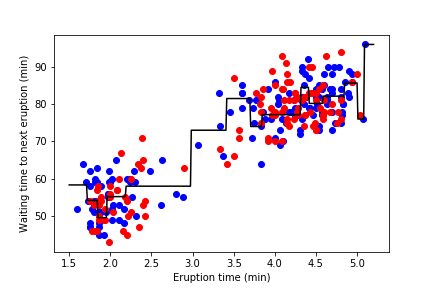
\includegraphics[width=0.9\textwidth]{dataplot.png}
	\end{centering}
\end{figure}

We also calculate the RMSE for several pre-pruning parameters, and here is our observation:
\begin{figure}[h]
	\centering
	\caption{RMSE versus Pre-pruning Parameter}
	\label{kernelfig}
	\begin{centering}
		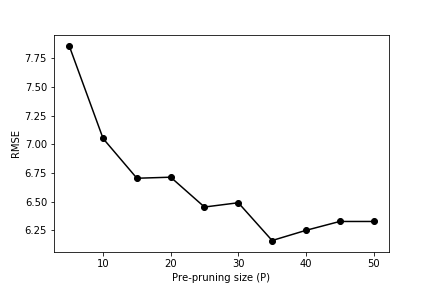
\includegraphics[width=0.9\textwidth]{pptorms.png}
	\end{centering}
\end{figure}

\end{document}